\documentclass[12pt,twoside,final]{article}

\usepackage[portuguese,brazil]{babel}
\usepackage[utf8]{inputenc}



%\usepackage{indentfirst, natbib}
\usepackage{indentfirst}

\usepackage{hyperref,ae}
% \usepackage{harvard}
\usepackage{pslatex}  %fonte times new roman
\usepackage{amssymb,fancyhdr,fancybox,epsfig,psfrag,amsmath,tabularx}
\usepackage[paperwidth=8.5in,paperheight=11in,hmargin={25mm,20mm},vmargin={20mm,20mm}]{geometry} %tamanho letter
\usepackage{graphicx, url}
%\usepackage{subfigure,tocloft}

%\setlength{\cftsubsecnumwidth}{0pt}
%\renewcommand{\cftsubsecaftersnumb}{\hspace{1.5em}}
%\setlength{\cftsubsecindent}{0em}
%\setlength{\cftsubsubsecindent}{0em}

\usepackage{caption}
%\captionsetup{labelsep=endash}
%\DeclareCaptionLabelSeparator*{cap_travessao}{--}

\usepackage{multirow}
\usepackage[lined,ruled,vlined,linesnumbered,portuguese]{algorithm2e}
\usepackage{ulem,soul}
\usepackage[dvips]{lscape} %rotacionar
\usepackage{setspace}
\usepackage{color}
\usepackage{wrapfig, graphics,multirow}
\usepackage{array}
\usepackage[dvipsnames,svgnames,x11names,table,xcdraw]{xcolor} 
\usepackage{colortbl,caption}
\usepackage{pdfpages}
\usepackage{enumitem,comment}  
%\usepackage[titletoc,toc,page]{appendix}
\usepackage[titletoc,title]{appendix}
\usepackage{graphicx}
\usepackage{subcaption}

%\usepackage[title]{appendix}
%\newcommand{\source}[1]{\caption*{Source: {#1}}}
%\renewcommand{\appendixtocname}{Ap\^endices}
%\renewcommand{\appendixpagename}{Ap\^endices}

%Center T�tulo do S�mario
%\renewcommand{\cfttoctitlefont}{\normalfont\Large\bfseries\MakeUppercase}
\renewcommand{\cfttoctitlefont}{\hspace*{\fill}\large\bfseries\MakeUppercase}
\renewcommand{\cftaftertoctitle}{\hspace*{\fill}}
%Center T�tulo do 
\renewcommand{\cftlottitlefont}{\hspace*{\fill}\large  \bfseries}
\renewcommand{\cftafterlottitle}{\hspace*{\fill}}
%Center T�tulo da Lista de Figuras 
\renewcommand{\cftloftitlefont}{\hspace*{\fill}\large \bfseries}
\renewcommand{\cftafterloftitle}{\hspace*{\fill}}


%\renewcommand{\listfigurename}{LIST OF FIGURES}
%\renewcommand{\listtablename}{LIST OF TABLES}

%\renewcommand\listtablename{LISTA DE TABELA}



\definecolor{lightgray}{gray}{0.8}
\definecolor{mediumgray}{gray}{0.75}

\usepackage[color]{showkeys}
\definecolor{refkey}{rgb}{0.39,0.58,1}
\definecolor{labeled}{rgb}{1,0,0}
\usepackage[Lenny]{fncychap}
\setlength{\headheight}{15pt}
\setlength{\parindent}{1.2cm}
\usepackage[num,abnt-repeated-author-omit=yes,abnt-emphasize = bf]{abntex2cite}
%=========================================== Headers =========================================

% \renewcommand{\chaptermark}[1]{\markboth{\chaptername\ \thechapter. \ #1}{ }}
\renewcommand{\sectionmark}[1]{\markright{\thesection. \ #1}}
\fancyhead{}
\fancyfoot{}
\fancyhead[RE,RO]{\thepage}
\renewcommand{\headrulewidth}{0pt}
%\fancyhead[RE]{\nouppercase{\leftmark}}
%\fancyhead[LO]{\nouppercase{\rightmark}}
%==============================================================================================

\hyphenation{pro-fis-si-o-nais}

% \input{macros}
\newcolumntype{P}[1]{>{\centering\arraybackslash}p{#1}}


\renewcommand{\listtablename}{LISTA TABELAS} 
\renewcommand{\listfigurename}{LISTA  FIGURAS}

%\defbibheading{bibliography}{\centering The New Name}

\begin{document}


\thispagestyle{empty}


%PPC em portugu�s
%================================================================================================
%================================= PRIMEIRA FOLHA INTERNA  ======================================
%================================================================================================
\begin{figure}
\center

\includegraphics[height=0.15\textwidth]{Figs/logoCefetCampusPetropolis.jpg} 
\end{figure}


\vspace*{0.8cm}

\begin{center}
{\large \bf CENTRO FEDERAL DE EDUCAÇÃO TECNOLÓGICA} \vspace{1mm} \\
{\large \bf CELSO SUCKOW DA FONSECA - CEFET/RJ \textit{CAMPUS} PETRÓPOLIS} \vspace{1mm} \\
{\large \bf CURSO: BACHARELADO EM ENGENHARIA DA COMPUTAÇÃO}

\vspace*{5cm}
{\large \bf NUTRIPIC \todo{Adicionar subtítulo. Algo do tipo: uma ferramenta/sistema/etc para pontuação de comida}} \\
\end{center}
\vspace{4cm}
\hfill
%\begin{minipage}%{0.45\linewidth}
	\begin{flushright}
	Isabella Grimaldi Gusmão \\
	Victoria Ribeiro Rodrigues
	\end{flushright}
%\end{minipage}


\vspace*{3.3cm}
\begin{center}
{\bf PETRÓPOLIS \\ 2018}\\
\end{center}

%--------------------------------------------------------------------------
%--------------------------------------------------------------------------
\newpage
\pagestyle{empty}

\begin{center}
{\large \bf CENTRO FEDERAL DE EDUCAÇÃO TECNOLÓGICA} \vspace{1mm} \\
{\large \bf CELSO SUCKOW DA FONSECA - CEFET/RJ \textit{CAMPUS} PETRÓPOLIS} \vspace{1mm} \\
{\large \bf CURSO: BACHARELADO EM ENGENHARIA DA COMPUTAÇÃO}

\vspace*{3cm}
\normalsize{\large \bf NUTRIPIC}\\
\end{center}
\vspace{1.5cm}
\hfill
%\begin{minipage}%{0.45\linewidth}
	\begin{flushright}
	Isabella Grimaldi Gusmão \\
	Victoria Ribeiro Rodrigues
	\end{flushright}
%\end{minipage}
\vspace*{1.5cm}
\begin{flushright}
	\begin{minipage}{0.5\textwidth}
		{\normalsize
		Trabalho de Conclusão de Curso apresentado ao  
	 CEFET/RJ -{\it campus} Petrópolis, como parte dos requisitos para obtenção do título de Bacharel em Engenharia da Computação.}
	\end{minipage}\\[1.5cm]
\end{flushright}
\vspace{1.5cm}
\hfill
%\begin{minipage}%{0.45\linewidth}
\begin{flushright}
Orientador: Prof. Douglas de Oliveira Cardoso
\end{flushright}




\vspace*{3.3cm}
\begin{center}
{\bf PETRÓPOLIS \\ 2018}\\
\end{center}



%--------------------------------------------------------------------------
%--------------------------------------------------------------------------
\newpage
\begin{minipage}{0.9\textwidth}

{\normalsize 
\begin{center}
Autorizo(amos) a reprodução e divulgação total ou parcial deste trabalho, por qualquer meio
eletrônico ou convencional, para fins de estudo e pesquisa, desde que citada a fonte.
\end{center}
\vspace*{0.5cm}
\begin{comment}
\begin{center}
ou
\end{center}
\vspace*{0.5cm}
\begin{center}
Nenhuma parte deste trabalho pode ser reproduzida ou divulgada, em qualquer meio eletrônico ou 
convencional, sem autorização do(s) autor(es). 
\end{center}
\end{comment}
}
\end{minipage}
\vspace*{5cm}
\begin{center}
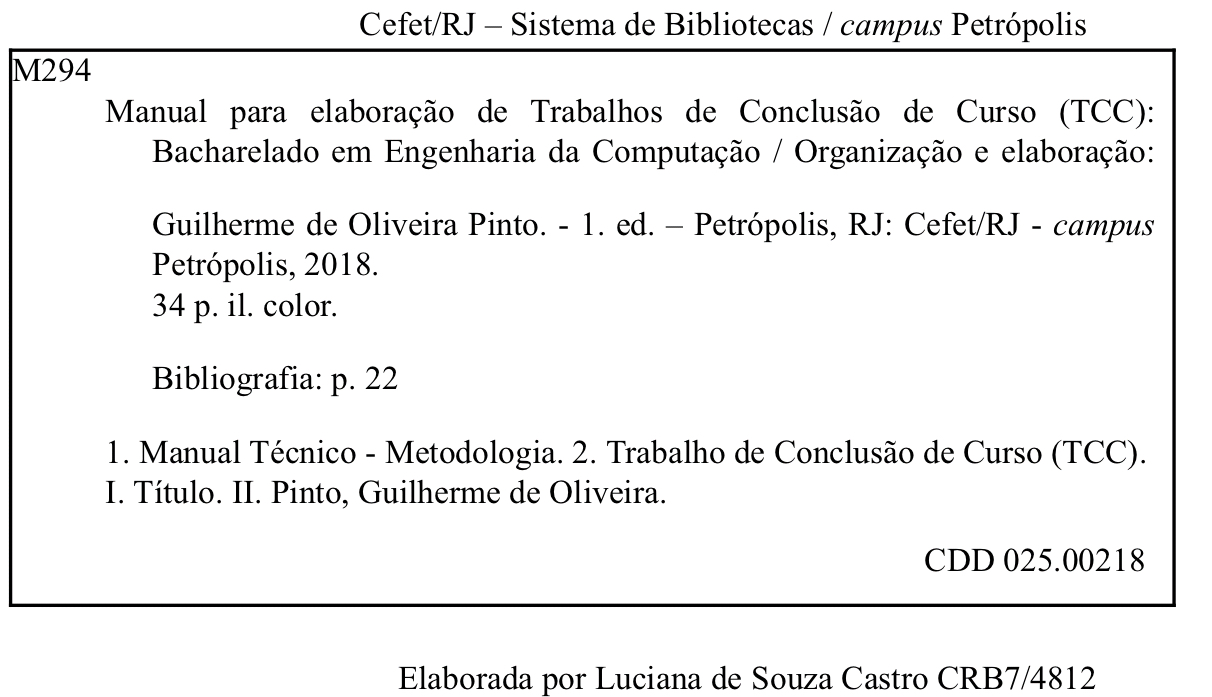
\includegraphics[height=0.4\textwidth]{Figs/biblioteca_engcomp.jpeg} \todo{Verificar com a biblioteca como se dá a confecção dessa imagem.}
\end{center}






%--------------------------------------------------------------------------
%--------------------------------------------------------------------------

\newpage
\newcommand{\HRule}{\rule{0.6\linewidth}{0.5mm}}
\pagestyle{empty}

{\center % Center everything on the page


\begin{figure}
\center

\includegraphics[height=0.13\textwidth]{Figs/logoCefetCampusPetropolis.jpg} 
\end{figure}

\begin{center}
{\large \bf CENTRO FEDERAL DE EDUCAÇÃO TECNOLÓGICA} \vspace{1mm} \\
{\large \bf CELSO SUCKOW DA FONSECA - CEFET/RJ \textit{CAMPUS} PETRÓPOLIS} \vspace{1mm} \\
{\large \bf CURSO: BACHARELADO EM ENGENHARIA DA COMPUTAÇÃO}

\vspace*{1.2cm}
{\large  FOLHA DE APROVAÇÃO}

\vspace*{1.3cm}
{\large \bf NUTRIPIC }\\
\end{center}
\vspace{0.5cm}
\hfill
%\begin{minipage}%{0.45\linewidth}
\begin{flushright}
    Isabella Grimaldi Gusmão \\
	Victoria Ribeiro Rodrigues
	\end{flushright}
%\end{minipage}
\vspace*{0.5cm}
\begin{flushright}
	\begin{minipage}{0.5\textwidth}
		{\normalsize
		Trabalho de Conclusão de Curso apresentado ao  
	 CEFET/RJ -{ {\it campus} Petrópolis}, como parte dos requisitos para obtenção do título de Bacharel em Engenharia da Computação.}
	\end{minipage}\\[0.5cm]
\end{flushright}
\vspace{0.5cm}
\hfill
%\begin{minipage}%{0.45\linewidth}
\begin{flushright}
Orientador: Prof. Douglas de Oliveira Cardoso
\end{flushright}

\begin{minipage}{0.9\textwidth}
	\begin{flushleft}
	Aprovado por:
	\end{flushleft}
\end{minipage}\\[1cm]

\center
\HRule \\
Prof. Douglas de Oliveira Cardoso, D.Sc. (Orientador) \\[1cm]
\HRule \\
Fulano da Silva, D.Sc. (Co-orientador)\\[1cm]
\HRule \\
Profa. Fulana da Silva, D.Sc.  \\[1.5cm]


\begin{center}
{Dezembro de 2018}
\end{center}


}



\newpage


% Dedicat�ria
\begin{center}
\textbf{\large DEDICATÓRIA}
\end{center}
      \vspace{0.5cm}

Opcional.
\newpage



% Agradecimento
\begin{center}
\textbf{\large  AGRADECIMENTO}
\end{center}
      \vspace{0.5cm}

Sempre haverá. Se não estiver inspirado, aqui está uma sugestão: dedico este trabalho ao povo brasileiro que contribuiu de forma significativa à minha formação e estada nesta Universidade. Este projeto é uma pequena forma de retribuir o investimento e confiança em mim depositados.
\newpage


% Resumo
\begin{center}
\textbf{\large RESUMO}
\end{center}
      \vspace{0.5cm}

Inserir o resumo do seu trabalho aqui. O objetivo é apresentar ao pretenso leitor do seu Projeto Final uma descrição genérica do seu trabalho. Você também deve tentar despertar no leitor o interesse pelo conteúdo deste documento.
\begin{flushleft}
{\bf Palavras-chaves:} Processamento de imagens. Inteligência computacional.
\end{flushleft}

\newpage

\begin{center}
\textbf{\large ABSTRACT}
\end{center}
\vspace{0.5cm}

Inserir o resumo do trabalho aqui, na Língua Inglesa.


\begin{flushleft}
{\bf Key-words:} Image Processing. Artificial Intelligence.
\end{flushleft}

\newpage

%=============================== lista de tabelas e figuras ==========================
{\thispagestyle{empty}
\renewcommand{\listfigurename}{LISTA DE FIGURAS}

\listoffigures}
\newpage

{\thispagestyle{empty}
\renewcommand{\listtablename}{LISTA DE TABELAS}
\listoftables}
\newpage

\begin{center}
\textbf{\large LISTA DE SIGLAS}
\end{center}
      \vspace{0.5cm}

\singlespacing

\noindent
\begin{tabular}{l c p{.85\linewidth}}

TCC & - & Trabalho de Conclusão de Curso \\
CEFET & - & Centro Federal de Educação Tecnológica \\
SWOT  & - &  {\it Strengths, Weaknesses, Opportunities, and Threats}\\


\end{tabular}

\onehalfspacing

\newpage

%=============================== sum�rio =============================================

\tableofcontents

\newpage
%caso o sum�rio acabe em uma p�gina �mpar, o verso ser� em branco
%\null \vfill
%\newpage

%Agora muda para o estilo fancy
\pagestyle{fancy}
\pagenumbering{arabic}
\setcounter{page}{12}
\onehalfspacing

\newpage
\section{Introdução\label{sec:intro}}

\subsection{Motivação\label{subsec:motiv}}

% O que justifica fazer esse trabalho?
% Quem ou o que é beneficiado por esse trabalho?
% qual a importância disso que queremos fazer?

\subsection{Objetivo\label{subsec:obj}}

% O que queremos fazer?
% O que NÃO queremos fazer
% escopo do trabalho

\subsection{Organização do Texto\label{subsec:org_texto}}


\subsection{Tema}


%Comentário
\begin{comment}
Falar do que se trata o trabalho usando uma visão macroscópica.

Sobre que grande área de conhecimento você vai falar?

Dada esta grande área, qual é o subconjunto de conhecimento sobre o qual será o seu trabalho?

Qual o problema a ser resolvido?
\end{comment}


O tema do trabalho é avaliar o quão saudável uma refeição individual é. Para isso vamos definir uma medida relativa a qualidade de um prato, que pode ser calculada diretamente a partir de seus ingredientes, e cujo valor deverá ser inferido a partir da imagem do próprio prato. Para isto serão empregadas técnicas de visão computacional e aprendizado de máquina. Estas técnicas serão combinadas em um aplicativo para dispositivos móveis, que tornará o processo de avaliação nutricional de refeições diárias mais rápido e prático.


\subsection{Delimitação}


%%%%Comentário

\begin{comment}
Realizar uma delimitação informando de quem é a demanda, em que local, e em que momento no tempo. Eventualmente, pode ser mais fácil começar pensando por exclusão, ou seja, para quem não serve, onde não deve ser aplicado, e em seguida pegar o universo que sobra.
\end{comment}

O funcionamento do aplicativo será baseado em imagens obtidas a partir da câmera do dispositivo móvel. Dessa forma, o desempenho do aplicativo dependerá da qualidade da câmera do aparelho. É importante ressaltar que o aplicativo não se propõe a fazer uma análise nutricional detalhada, como faria um profissional da área. As funcionalidades a serem implementadas serão baseadas em exemplos de refeições previamente analisadas. Sendo assim, sua utilidade será limitada a outras refeições nos mesmos moldes destes exemplos, os quais não contemplam refeições coletivas ou dispostas de forma incomum.


\subsection{Justificativa}
%%%%ler o comentário
\begin{comment}
Apresentar o porquê do tema ser interessante de ser estudado. Cuidado, não é a motivação particular. Devem ser apresentadas razões para que alguém deva se interessar no assunto, e não quais foram suas razões particulares que motivaram você a estudá-lo.
\end{comment}


%MOTIVO 1: MELHORIA DA VIDA HUMANA
A tecnologia sempre esteve presente na vida dos seres humanos. Com o passar dos anos, foram criadas mais e mais ferramentas para tornar nossas vidas mais práticas. Com estas ferramentas podemos facilitar muito nossas atividades. É impossível negar a utilidade dos telefones móveis. Podemos nos comunicar, cuidar da nossa saúde, trabalhar, entender o mundo a nossa volta e alcançar nossas metas.%TODO: A ÙLTIMA FRASE DESTE PARÀGRAFO PARECE FORA DO CONTEXTO. CABE VERIFICAR.

Para tratar as mais distintas necessidades humanas, aplicativos para celular estão sendo desenvolvidos, de forma personalizada. Existem aplicativos para controle de finanças, os que auxiliam no controle de dietas, os que ajudam a controlar os estudos e muitos outros mais. Embora não seja recomendado passar horas utilizando o celular, é sim uma boa ideia saber usá-lo da melhor forma possível.

%MOTIVO 2: UTILIDADE DE APPS SIMILARES
Aplicativos de contagem de calorias são uma das ferramentas que surgiram com o advento de aplicativos que auxiliam no registro e controle das refeições diárias. Eles são recomendados para quem quer controlar a ingestão de calorias, seja para emagrecer ou acompanhar alterações específicas da dieta. Os aplicativos ajudam a ter uma visão ampla e clara de como está sua alimentação \cite{payne2015behavioral}. Assim, é possível fazer ajustes para alcançar determinados objetivos. 

%MOTIVO 3: POSSIBILIDADE DE MELHORIA DE APPS EXISTENTES
A grande maioria desses aplicativos utiliza um filtro de busca através do qual conseguimos pesquisar cada componente da refeição e adicionar as quantidades desejadas. Porém, colocar um alimento por vez, torna a tarefa de contabilizar calorias demorada e nada prática. Entretanto nosso aplicativo busca atacar esse problema de forma diferente.

%Neste sentido, o presente projeto busca aprimorar essa contagem utilizando a câmera do dispositivo. Basta apontar a câmera do dispositivo para a sua refeição e tirar uma foto.

Neste sentido, o presente projeto busca aprimorar essa inserção de alimentos manualmente utilizando a câmera do dispositivo. Basta apontar a câmera do dispositivo para a sua refeição e tirar uma foto. 

Além disso, o projeto se propõe a avaliar uma refeição usando apenas informações visuais, buscando assim não se ater a considerar calorias ou outros valores nutricionais básicos, e também limitar-se a alimentos previamente registrados.


\subsection{Objetivos}

%%comentário
\begin{comment}
Informar qual é o objetivo geral do trabalho, isto é, aquilo que deve ser atendido e que corresponde ao indicador inequívoco do sucesso do seu trabalho. Pode acontecer que venha a existir um conjunto de objetivos específicos, que complementam o objetivo geral (tamanho do texto: livre, mas cuidado para não fazer uma literatura romanceada, afinal esta seção trata dos objetivos).
\end{comment}


Já existem no mercado alguns aplicativos que se propõem a identificar comidas e mostrar seus dados nutricionais.
Em alguns testes com um dos mais robustos, o Calorie Mama \cite{caloriemama_2016}, verificamos que podemos tirar foto do prato e, assim, ele nos mostra opções que se pareçam mais relevantes dados os alimentos que estão no prato, como mostra a Figura \ref{fig:test}.

Diferentemente dos aplicativos que estão no mercado, o objetivo deste trabalho é o desenvolvimento um aplicativo que permita avaliar quão saudável uma refeição individual é utilizando apenas uma imagem do prato. Através de reconhecimento de padrões, baseado num amplo banco de imagens de pratos de refeições com suas respectivas informações nutricionais, será possível informar se o prato é ou não saudável possivelmente considerando atributos como variedade de elementos no prato, coloração do prato, além de outras características ocultas, inferidas a partir de exemplos de fotos de refeições cujos ingredientes e outras informações foram indicadas manualmente \cite{nasrabadi2007pattern}.


\begin{figure}[!ht]
\centering
\caption{Comparação entre diferentes pratos.}
\begin{subfigure}{0.4\textwidth}
  \centering
    \caption{Prato com comidas japonesas.}
   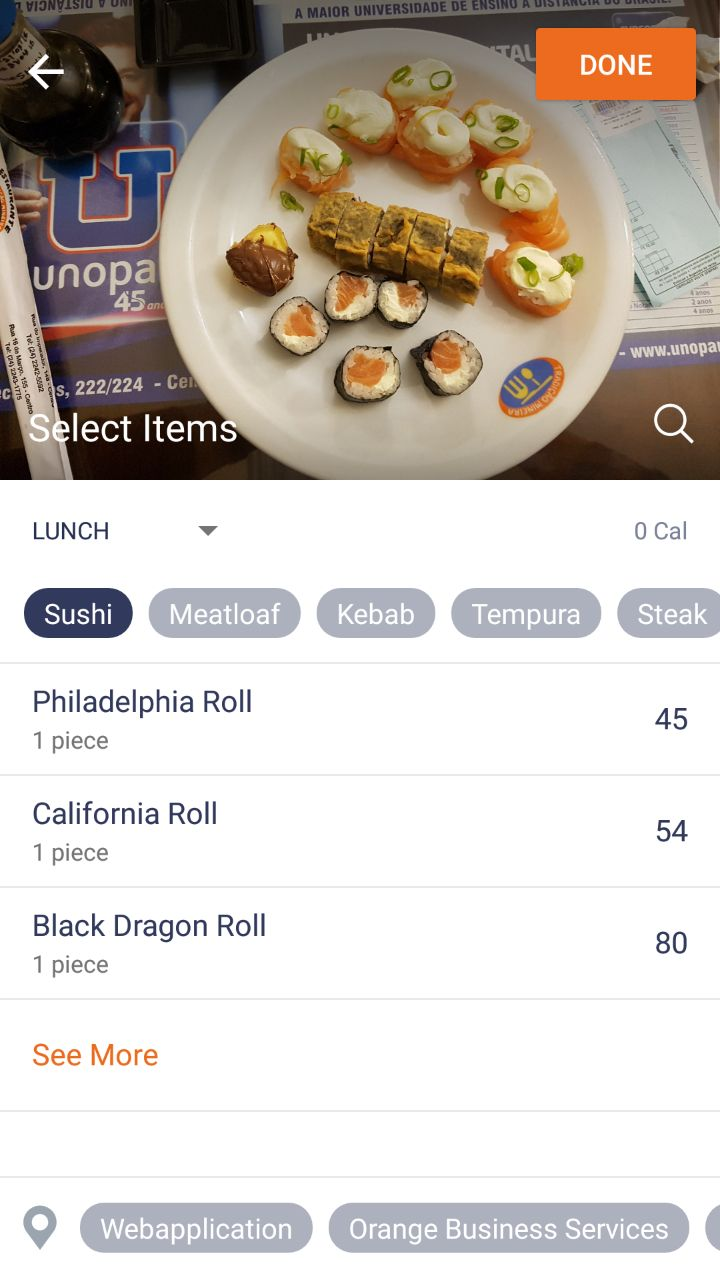
\includegraphics[width=\textwidth]{imgs/sushi.jpeg}
  \label{fig:sub1}
\end{subfigure}%
\hspace{.1\textwidth}
\begin{subfigure}{0.4\textwidth}
  \centering
    \caption{Prato com comidas brasileiras.}
  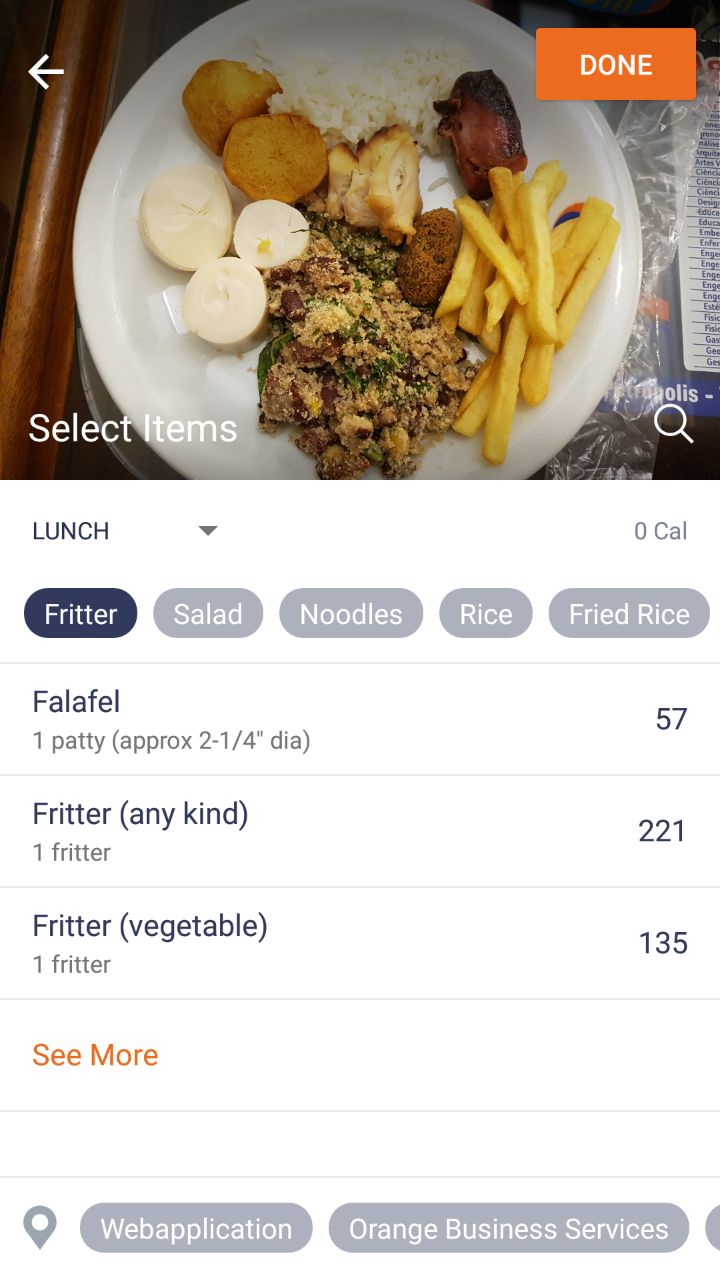
\includegraphics[width=\textwidth]{imgs/brasileira.jpeg}
  \label{fig:sub2}
\end{subfigure}

\label{fig:test}
\end{figure}



\subsection{Metodologia}

%%% comentário
\begin{comment}
Como é a abordagem do assunto. Como foi feita a pesquisa, se vai houve validação, etc. Em resumo, você de explicar qual foi sua estratégia para atender ao objetivo do trabalho.
\end{comment}

Para o aplicativo móvel, implementaremos uma interface simples e de fácil entendimento ao usuário final. Escolhemos o React-Native \cite{react-native_2015} pois permite o desenvolvimento simultâneo para Android e iOS, os sistemas operacionais que dominam o mercado de dispositivos móveis. 

Utilizaremos redes neurais treinadas usando conjuntos de dados com dezenas de milhares de imagens de refeições \cite{kawano2014food}. Por se tratar de um problema com muitas dimensões a serem consideradas, é necessário um grande conjunto de treinamento. Esses conjuntos de dados já estão anotados, contendo indicações de informações dos alimentos presentes na fotografia. Não é necessário se preocupar em ruídos na imagem, como a superfície na qual o objeto se encontra, talheres e o próprio prato. É esperado que o método de aprendizado descarte esses detalhes.
Ao reconhecer o alimento, determinaremos algumas informações nutricionais e outras medidas, como quão colorido é o prato, para podemos informar de alguma forma se o prato é saudável ou não.

\subsection{Organização do texto}

No capítulo 2 será apresentada a base para o estudo de leitura labial, e 

O capítulo 3 apresenta ...

Os .... são apresentados no capítulo 4. Nele será explicitado ...

E assim vai até chegar na conclusão.

\section{Trabalhos Relacionados \label{sec:trab_rel}}

\subsection*{Introdução}

\subsubsection*{Descrição geral do que tratará esta seção}
\subsubsection*{Organização desta seção}

\subsection{Aplicativos, websites e sistemas em geral \label{subsec:app_web}}

Devido ao aumento do poder computacional devido ao advento das Unidades de Processamento Gráfico (GPUs), o uso de Redes Neurais para identificar objetos em imagens tornou-se viável.

Empresas como Google, Amazon e Microsoft, juntaram suas pesquisas em reconhecimento de imagem em APIs (Application Programming Interfaces) para que os desenvolvedores de software possam usar essa tecnologia em aplicativos. As APIs são as seguintes: Google Vision API \cite{google_vision}, Amazon Rekognition \cite{amazon_rekognition}, e Microsoft Computer Vision API \cite{azure_microsoft_computer_vision}.

Aplicativos de perda de peso, em que há um acompanhamento das refeições feitas durante o dia, existem há anos, mas exigiam que os usuários inserissem manualmente o que estavam comendo em seus bancos de dados para rastrear as calorias e os valores nutricionais dos alimentos. Hoje em dia, existem softwares que já fazem o reconhecimento de imagens e são capazes de identificar o alimentos presentes em uma foto.

O Calorie Mama \cite{caloriemama_2016} é um aplicativo para celular que promete exatamente isso. Basta tirar uma foto da comida para obter as informações nutricionais da refeição. O Calorie Mama utiliza o Food AI API para reconhecimento dos itens alimentares nas imagens.

O aplicativo Lose It \cite{lose_it} também promete a mais avançada tecnologia de reconhecimento de imagem para oferecer a melhor experiência de rastreamento de alimentos no mundo através de um recurso chamado Snap It.

A figura \ref{fig:apps} mostra o funcionamento dos dois aplicativos. A figura \ref{fig:subApps1} mostra a tela do Calorie Mama, onde a figura utilizada foi de um prato de macarrão. Percebe-se que a sugestão dada pelo aplicativo é a categoria "pasta" que significa "massa" em português. O mesmo acontece para a figura \ref{fig:subApps2}, em que é utilizada a mesma imagem, mas no Lose It e a categoria que foi sugerida pelo aplicativo é também "pasta".

\begin{figure}[!ht] 
\centering
\caption{Comparação entre os aplicativos.}
\label{fig:apps}
\begin{subfigure}{0.4\textwidth}
  \centering
    \caption{Aplicativo Calorie Mama.}
   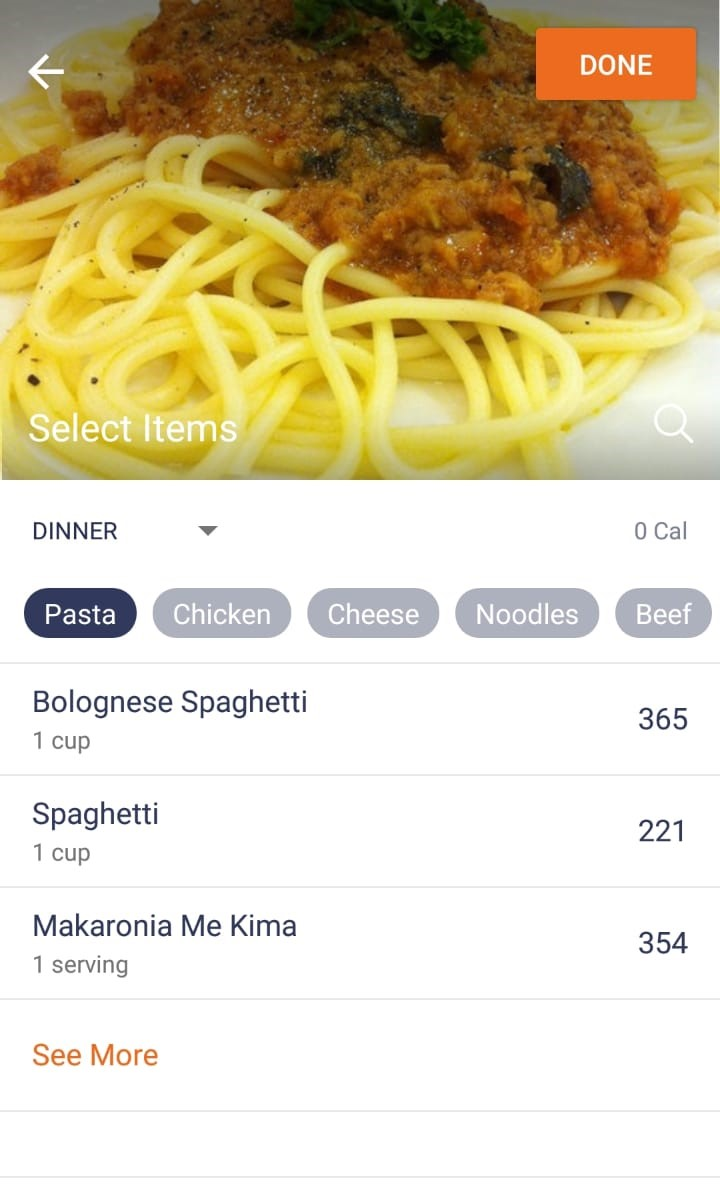
\includegraphics[width=\textwidth]{imgs/mama.jpeg}
  \label{fig:subApps1}
\end{subfigure}%
\hspace{.1\textwidth}
\begin{subfigure}{0.4\textwidth}
  \centering
    \caption{Aplicativo Lose It.}
  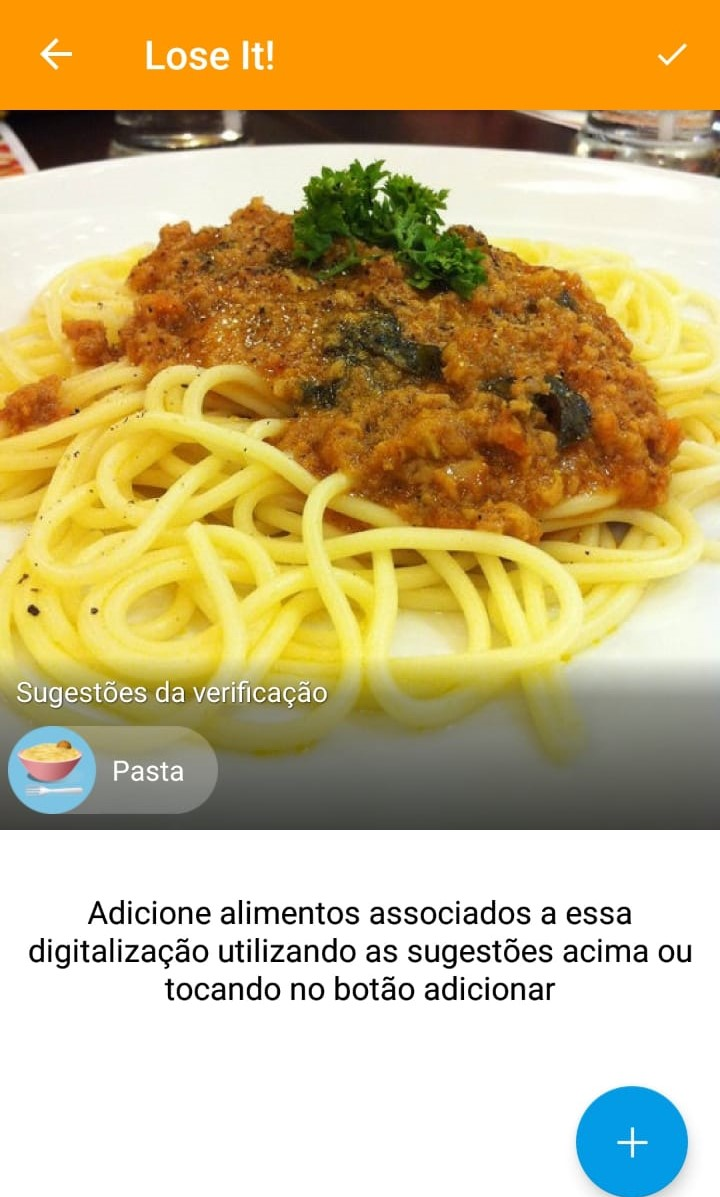
\includegraphics[width=\textwidth]{imgs/loseit.jpeg}
  \label{fig:subApps2}
\end{subfigure}

\label{fig:test}
\end{figure}


\subsection{Redes Neurais Artificias etc \label{subsec:nn}}

Redes Neurais Artificiais (RNA) são estruturas computacionais inspiradas no sistema nervoso de seres vivos. Essas estruturas
Neste capítulo, são apresentados alguns dos métodos detecção e reconhecimento de alimentos através de imagens. O objetivo aqui é descrever as vantagens e principais desvantagens desses métodos e seus respectivos resultados. 


\subsection{Detecção e Reconhecimento de Imagens}
A detecção e reconhecimento de imagens contendo alimentos são tópicos frequentemente pesquisados na área de visão computacional. Existem vários artigos publicados com diferentes abordagens para resolver esses dois problemas.  

\subsubsection{Detecção de Alimentos em Imagem}
A detecção de alimentos é diferente do reconhecimento alimentos, pois a primeira é uma classificação binária de imagens em imagens alimentares e não-alimentares, isto é, se contém comida ou não. Dada uma imagem, em que pode conter comida e fundo, a detecção de alimentos classifica a imagem como alimentar ou não-alimentar.

A Rede Neural Convolucional (CNN) oferece a mais recente técnica para muitos problemas gerais de classificação de imagem. Kagaya \cite{kagaya2014food} aplicou a CNN na classificação alimentar/não-alimentar e obteve resultados significativos com uma acurácia de 93,8\%. E, no trabalho \cite{kagaya2015highly}, a acurácia na detecção de alimentos foi aumentada para 99,1\%.

Esses resultados expressam que, em relação a trabalhos anteriores que utilizavam abordagens convencionais de aprendizado de máquina, a utilização de CNN aparenta mostrar uma melhor performance.

\subsubsection{Reconhecimento de Alimentos em Imagem}
A maioria dos trabalhos de pesquisa em reconhecimento de alimentos assumem que apenas um alimento está presente na imagem. Assim, o reconhecimento de alimentos pode ser resolvido como um problema de classificação multi-classes. 

A CNN também é amplamente utilizada no reconhecimento de alimentos e fornece melhor desempenho do que os métodos convencionais. 

Kagaya \cite{kagaya2014food} também treinou uma CNN para reconhecimento de alimentos e os resultados experimentais mostraram que a CNN superou todas as outras abordagens clássicas alcançando uma acurácia média de 73,7\% para 10 classes. Singla \cite{singla2016food} aplicou um modelo GoogLeNet pré-treinado baseado na arquitetura CNN nas tarefas de classificação de imagens alimentares/não-alimentares e para reconhecimento de categoria de alimentos. Os resultados experimentais mostram a precisão geral de 99,2\% na classificação alimentar/não-alimentar e 83,6\% na categorização de alimentos. 

A detecção e identificação de alimentos tem sido investigada na literatura em diferentes trabalhos, como os citados acima, inclusive \cite{aguilar2017food} e \cite{pouladzadeh2017cloud} em que foi evidenciado que os melhores resultados obtidos são baseados em Redes Neurais Convolucionais (CNN).







\section{Atribuição de valor a imagens de refeições}

\subsection{Arquitetura do sistema}

Para o trabalho utilizamos um desktop com 32GB de RAM i7-4790K CPU @ 4.00GHz com placa de vídeo GeForce GTX 980.

\subsubsection{TensorFlow}

O aprendizado de máquina é uma disciplina complexa. Porém, hoje, a implementação de modelos de aprendizado de máquina é mais simples do que costumava ser, graças aos frameworks de aprendizado de máquina, como o TensorFlow, que facilitam o processo de aquisição de dados, modelos de treinamento, previsões e refinamento de resultados futuros.

%https://www.infoworld.com/article/3278008/tensorflow/what-is-tensorflow-the-machine-learning-library-explained.html

%https://aws.amazon.com/pt/tensorflow/

O TensorFlow é uma biblioteca de software de código aberto para computação numérica que usa gráficos de fluxo de dados. Os nós no gráfico representam operações matemáticas, e as arestas representam as matrizes ou tensores de dados multidimensionais que se comunicam com os nós. Essa arquitetura flexível permite a implantação de aplicações a uma ou mais CPUs ou GPUs em um desktop, servidor ou dispositivo móvel sem reescrever o código. O TensorFlow também inclui o TensorBoard, um kit de ferramentas de visualização de dados. O TensorBoard é um conjunto web de aplicativos para inspecionar e entender suas execuções e gráficos do TensorFlow.

O TensorFlow foi desenvolvido originalmente por pesquisadores e engenheiros que trabalham na equipe do Google Brain, na organização Machine Intelligence Research do Google, com o objetivo de realizar pesquisas sobre redes neurais profundas e aprendizado de máquina. Ele fornece tudo para o programador por meio da linguagem Python. O Python é fácil de aprender e trabalhar. Nós e tensores em TensorFlow são objetos Python, e os aplicativos TensorFlow são aplicativos em Python.

As operações matemáticas reais, entretanto, não são executadas no Python. As bibliotecas de transformações que estão disponíveis através do TensorFlow são escritas como binários C ++ de alto desempenho. O Python apenas direciona o tráfego entre as partes e fornece abstrações de programação de alto nível para conectá-las.

O maior benefício que o TensorFlow oferece para o desenvolvimento de aprendizado de máquina é a abstração. Em vez de lidar com os detalhes básicos da implementação de algoritmos, ou de descobrir formas adequadas de ligar a saída de uma função à entrada de outra, o desenvolvedor pode se concentrar na lógica geral da aplicação. TensorFlow cuida dos detalhes nos bastidores.


\subsubsection{Keras}
Keras é uma API de redes neurais de alto nível, escrita em Python e capaz de rodar em cima do TensorFlow, CNTK ou Theano que pode rodar na CPU ou GPU.

Princípios orientadores

Facilidade de utilização: Keras é uma API projetada para seres humanos, não para máquinas. Coloca a experiência do usuário na frente e no centro. I Keras segue as práticas recomendadas para reduzir a carga cognitiva: ele oferece APIs consistentes e simples, minimiza o número de ações do usuário necessárias para casos de uso comuns e fornece um feedback claro e acionável sobre o erro do usuário.

Modularidade: Um modelo é entendido como uma sequência ou um gráfico de módulos autônomos configuráveis que podem ser conectados com o menor número de restrições possível. Em particular, camadas neurais, funções de custo, otimizadores, esquemas de inicialização, funções de ativação, esquemas de regularização são todos módulos independentes que você pode combinar para criar novos modelos.

Extensibilidade fácil: Novos módulos são simples de adicionar (como novas classes e funções), e os módulos existentes fornecem exemplos amplos. Poder criar facilmente novos módulos permite total expressividade, tornando Keras adequado para pesquisa avançada.

Trabalhe com o Python: Não há arquivos de configuração de modelos separados em um formato declarativo. Os modelos são descritos em código Python, que é compacto, mais fácil de depurar e permite a facilidade de extensibilidade.

Aplicações Keras são modelos de deep learning que são disponibilizados juntamente com pesos pré-treinados. Esses modelos podem ser usados para previsão, extração de recursos e ajuste fino.

%https://keras.io/#keras-the-python-deep-learning-library

\subsection{Modelos de redes neurais considerados e sua avaliação}


Os modelos disponíveis para classificação de imagens com pesos treinados no ImageNet são:

\begin{itemize}
    \item Xception
    \item VGG16
    \item VGG19
    \item ResNet50
    \item InceptionV3
    \item InceptionResNetV2
    \item MobileNet
    \item DenseNet
    \item NASNet
    \item MobileNetV2
\end{itemize}

Todas essas arquiteturas são compatíveis com todos os backends (TensorFlow, Theano e CNTK).

Os modelos utilizados nesse trabalho foram o MobileNetV2, DenseNet121 e o NASNetMobile.

\subsubsection{MobileNetV2}
Em 2017, um grupo de pesquisadores do Google publicou um artigo que apresentava uma arquitetura de rede neural otimizada para dispositivos móveis. Essa arquitetura chamada de MobileNets são modelos pequenos, com baixa latência e baixo consumo de energia parametrizados para atender às restrições de recursos de vários casos de uso. Eles podem ser construídos para classificação, detecção, incorporação e segmentação, semelhante a como outros modelos populares de grande escala, como o Inception, são usados. Os MobileNets podem ser executados de forma eficiente em dispositivos móveis com o TensorFlow Mobile.

%https://ai.googleblog.com/2017/06/mobilenets-open-source-models-for.html

%https://towardsdatascience.com/mobilenetv2-inverted-residuals-and-linear-bottlenecks-8a4362f4ffd5

A capacidade de executar redes profundas em dispositivos móveis pessoais melhora a experiência do usuário, oferecendo acesso a qualquer hora, em qualquer lugar, com benefícios adicionais para segurança, privacidade e consumo de energia. À medida que novos aplicativos surgem, permitindo que os usuários interajam com o mundo real em tempo real, o mesmo acontece com a necessidade de redes neurais cada vez mais eficientes. Por isso, a Google apresentou uma nova versão dessa arquitetura esse ano, o MobileNetV2.


O MobileNetV2 é uma melhoria significativa em relação ao MobileNetV1 e impulsiona o estado da arte para reconhecimento visual móvel, incluindo classificação, detecção de objetos e segmentação semântica. O MobileNetV2 baseia-se nas ideias do MobileNetV1, porém, a V2 introduz dois novos recursos à arquitetura: Resíduos Invertidos e Gargalos Lineares.

Em comparação com a primeira versão, no geral, os modelos do MobileNetV2 são mais rápidos com a mesma precisão em todo o espectro de latência. Em particular, os novos modelos usam duas vezes menos operações, precisam de 30\% menos parâmetros e são cerca de 30-40\% mais rápidos em um telefone do Google Pixel do que os modelos do MobileNetV1, tudo isso com maior precisão.

%https://ai.googleblog.com/2018/04/mobilenetv2-next-generation-of-on.html

\begin{figure}[!ht]
\centering 
\caption{O MobileNetV2 melhora a velocidade (latência reduzida) e aumenta a precisão do ImageNet Top 1}
\label{fig:mobilenetv1vsv2}
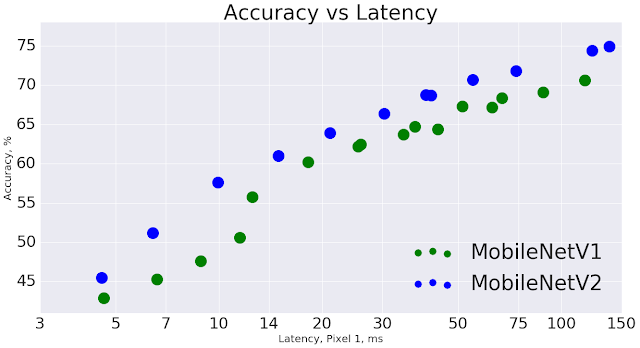
\includegraphics[width=0.9\textwidth]{imgs/mobilenetv1vsv2.png}
\end{figure}


\subsubsection{DenseNet121}

À medida que as CNNs se tornam cada vez mais profundas, surge um novo problema de pesquisa: conforme as informações sobre a entrada ou gradiente passam por várias camadas, elas podem desaparecer antes de chegar ao fim da rede.

%https://arxiv.org/pdf/1608.06993.pdf

Redes Convolucionais Densamente Conectadas (DenseNets) simplificam o padrão de conectividade entre camadas introduzidas em outras arquiteturas. Os autores resolvem o problema garantindo o fluxo máximo de informações (e gradientes). Para fazer isso, eles simplesmente conectam cada camada diretamente entre si. Em vez de extrair poder de representação de arquiteturas extremamente profundas ou amplas, as DenseNets exploram o potencial da rede por meio do reuso de recursos. As DenseNets requerem menos parâmetros que um CNN tradicional equivalente, já que não há necessidade de aprender mapas de recursos redundantes.

DenseNets, em contraste com ResNets, nunca combinam recursos por meio do somatório antes de serem passados para uma camada. Em vez disso, combinam recursos concatenando-os.
Assim, a camada l tem l entradas, consistindo nos mapas de características de todos os blocos convolucionais precedentes. Seus próprios mapas de características são passados para todas as camadas subsequentes de L-l. Isso introduz as conexões L (L + 1) 2 em uma rede de camada L, em vez de apenas L, como nas arquiteturas tradicionais. Devido ao seu denso padrão de conectividade, a abordagem foi chamada de Dense Convolutional Network (DenseNet).

\begin{figure}[!ht]
\centering 
\caption{Um bloco denso de 5 camadas com uma taxa de crescimento de k = 4. Cada camada usa todos os mapas de recursos anteriores como entrada.}
\label{fig:densenet}
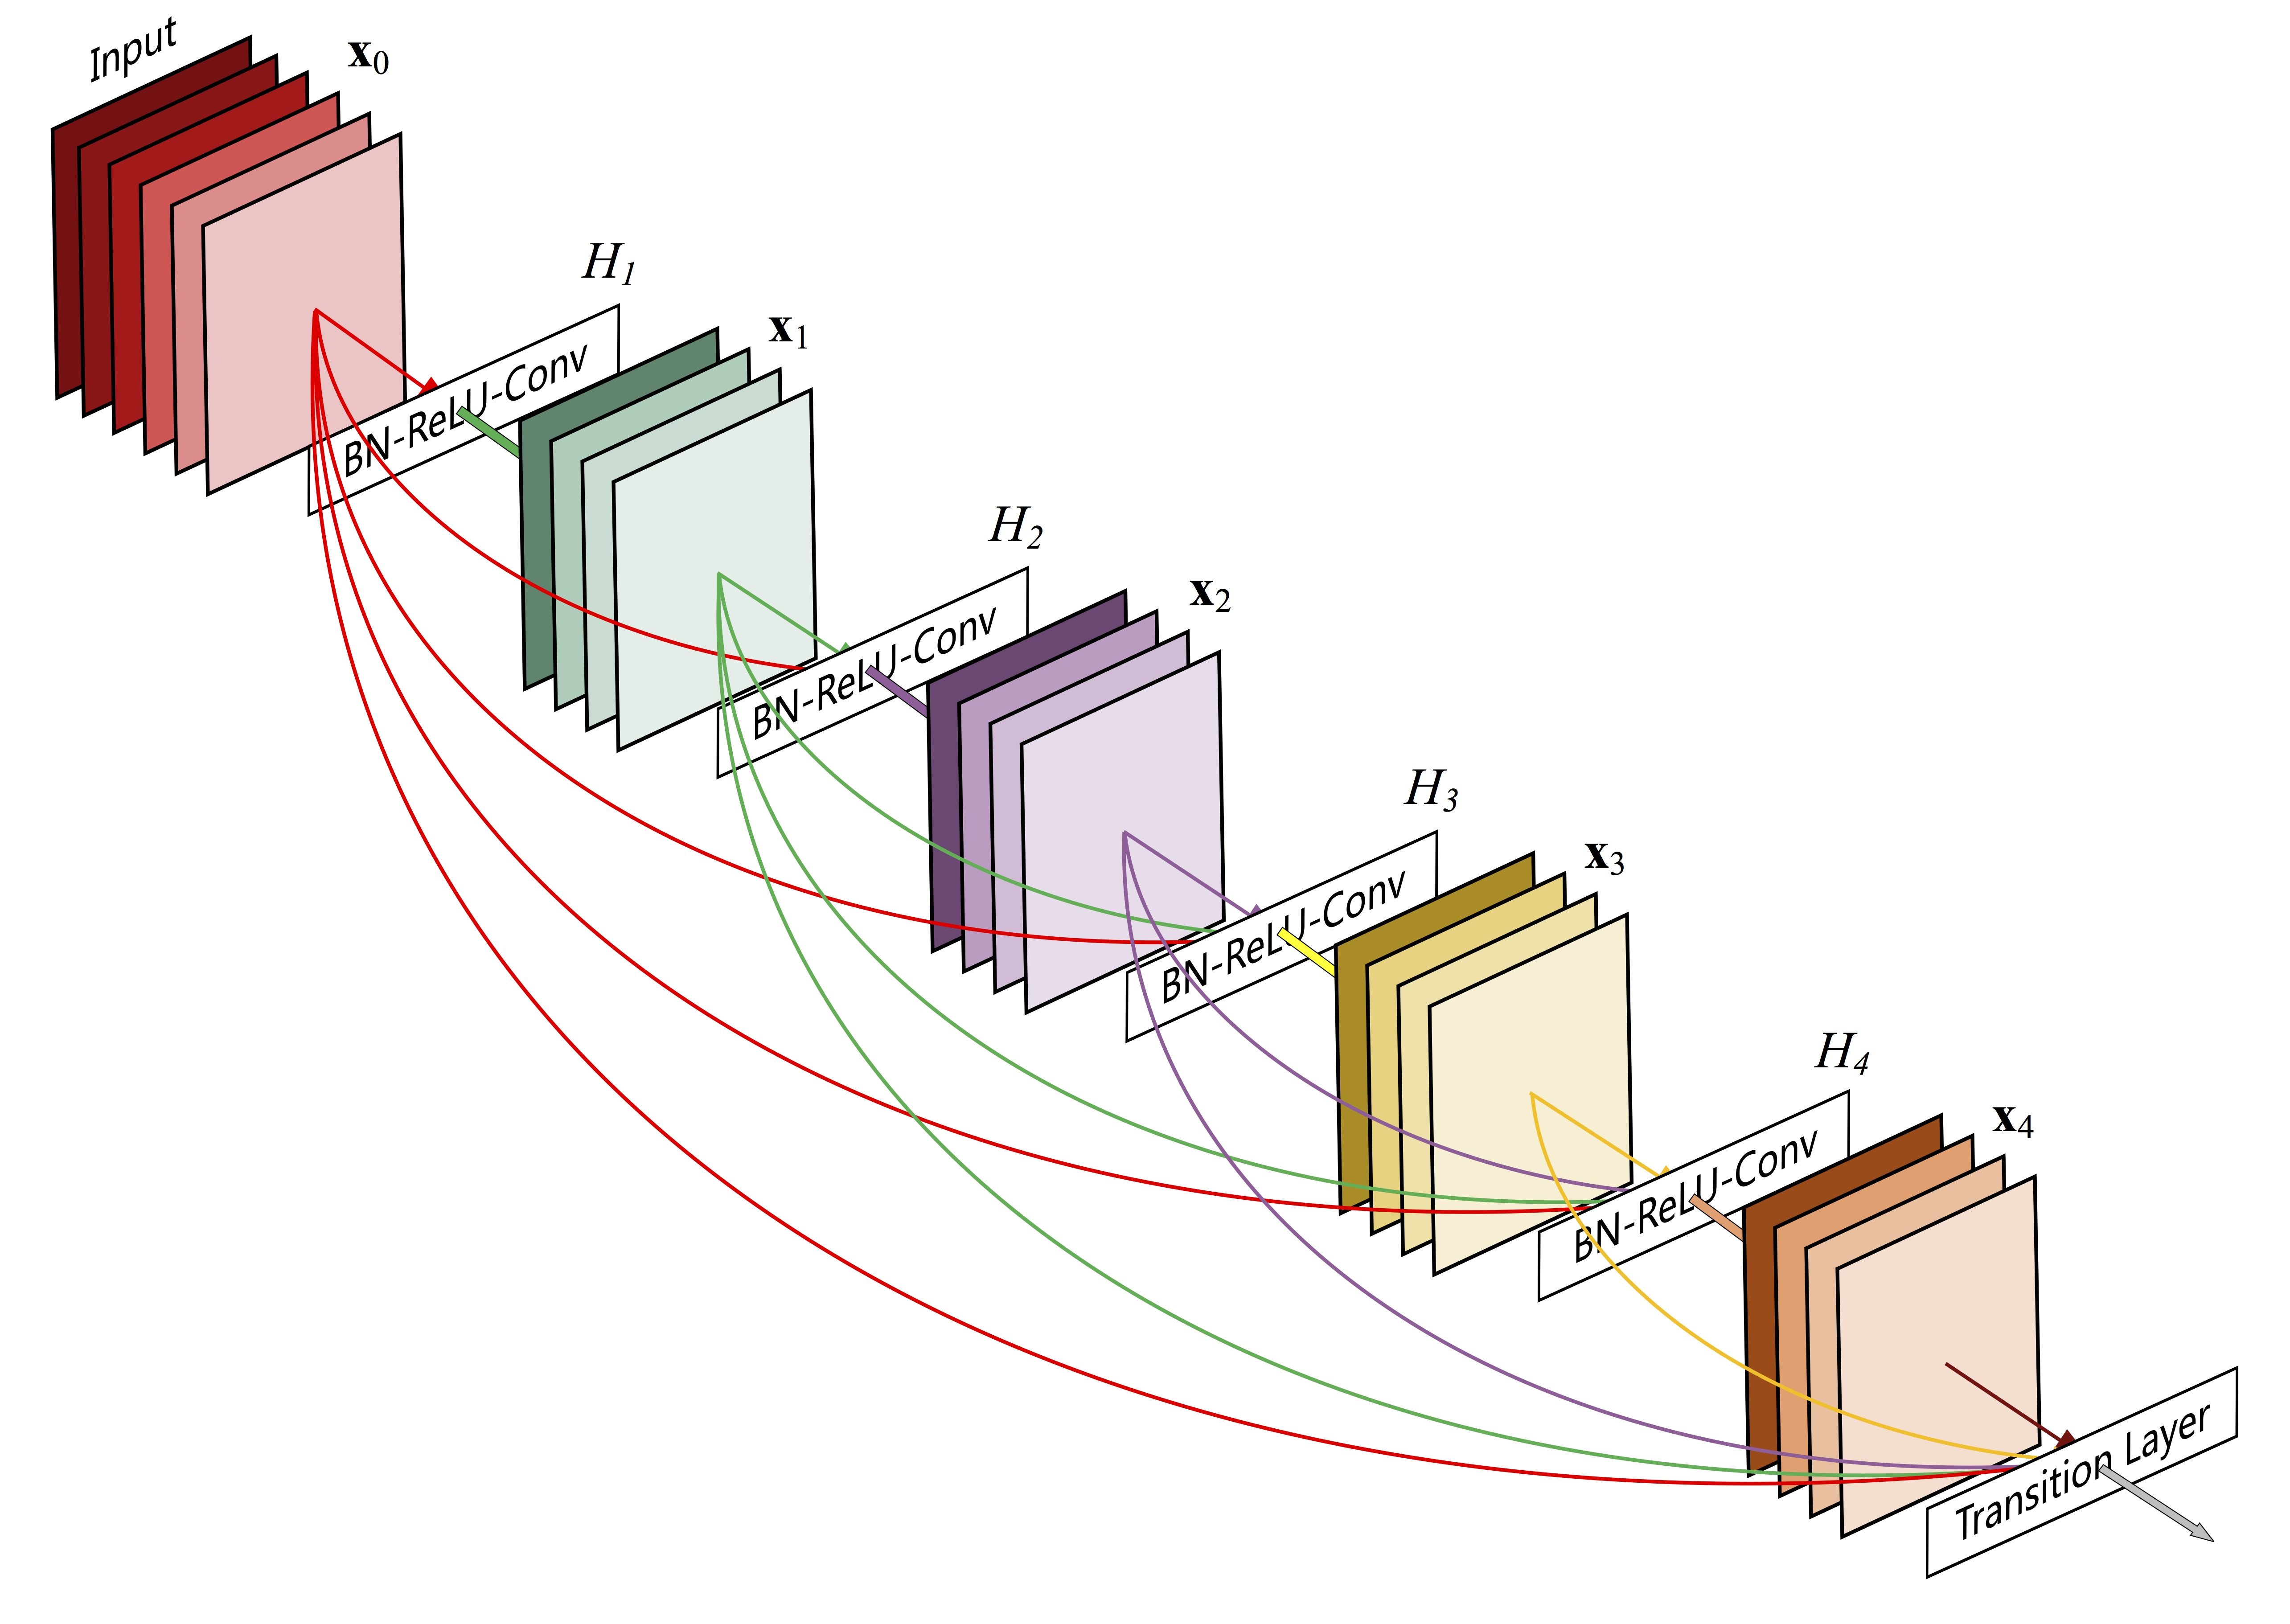
\includegraphics[width=0.9\textwidth]{imgs/densenets.jpg}
\end{figure}

\subsubsection{NASNetMobile}

%https://towardsdatascience.com/everything-you-need-to-know-about-automl-and-neural-architecture-search-8db1863682bf
\section{Resultados Obtidos}

\subsection{Aplicação para usuários finais}
\subsection{Kernel do sistema}
\section{Conclusão}
\subsection{Trabalhos Futuros}

\nocite{NBR6023,NBR6024,NBR6027,NBR6028,NBR10520,NBR14724,IBGE,CEFET_2007,CEFET_2014}


%@manual{CEFET_2014,
%address={Petrópolis (RJ)},
%organization={CELSO FEDERAL DE EDUCAÇÃO TECNOLÓGICO CELSO SUCKOW DA FONSECA. Campus Petrópolis. Coordenação de %Trabalho %de Conclusão de Curso},
%title={Manual para elaboração de Trabalho de Conclusão de Curso (TCC)},
%year={2014}
%}

%%% Bibliografia %%%
%\addcontentsline{toc}{section}{Refer�ncias}
%\bibliographystyle{apateste}

%\bibliographystyle{abnt-alf}
{
\thispagestyle{empty}
\renewcommand{\refname}{REFERÊNCIAS}
\bibliography{bibliografia}
}

\newpage
\begin{comment}
\begin{appendices}
%\renewcommand{\chaptername}{Ap�ndice}
\section{T�tulo do Ap�ndice} \label{ap:defesa}

\paragraph{}Elemento que consiste em um texto ou documento elaborado pelo autor, com o intuito de complementar sua, sem preju�zo do trabalho. S�o identificados por letras mai�sculas consecutivas e pelos respectivos t�tulos.
\section{T�tulo do Ap�ndice}

Documenta��o n�o elaborada pelo autor, ou elaborada pelo autor mas constituindo parte de outro projeto.
%\include{apendiceD}
\end{appendices}
\end{comment}

\end{document}